\documentclass[12pt,a4paper]{article}
\usepackage[utf8]{inputenc}
\usepackage[german]{babel}
\usepackage[T1]{fontenc}
\usepackage{amsmath}
\usepackage{amsfonts}
\usepackage{hyperref}
\usepackage{amssymb}
\usepackage{graphicx}
\usepackage{listings}
\usepackage[left=2cm,right=2cm,top=2cm,bottom=2cm]{geometry}

%%this removes empty ":" after abbildung 1:
\usepackage{caption}

\newtheorem{theorem}{Definition}
\author{Frank Leuchtmann}
\title{Systematische Generierung konsistenter Mengen qualitativer
Konditionale}

% this value solves the problem overfull hbox. it defines somehow max empty space in a line.
\tolerance=750

\newcommand{\lag}{\mathcal{L}}

%%the following 2 is to define the dotl command. can this be shorter??
\newcommand\dotl{\mathrel{%
    \mathchoice{\QEQ}{\QEQ}{\QEQ}{\QEQ}%
}}
\def\QEQ{{%
    \setbox0\hbox{<}%
    \rlap{\hbox to \wd0{\hss \raisebox {0.1pt}{$\ \cdot$\hss}}}\box0
}}

\newcommand\dotll{\mathrel{%
    \mathchoice{\QEQQ}{\QEQQ}{\QEQQ}{\QEQQ}%
}}
\def\QEQQ{{%
    \setbox0\hbox{$\leqslant$}%
    \rlap{\hbox to \wd0{\hss \raisebox {1pt}{$\ \cdot$\hss}}}\box0
}}

% rdotl command
\newcommand\rdotl{\mathrel{%
    \mathchoice{\RQEQ}{\RQEQ}{\RQEQ}{\RQEQ}%
}}
\def\RQEQ{{%
    \setbox0\hbox{$\prec$}%
    \rlap{\hbox to \wd0{\hss \raisebox {0.01pt}{$\ \cdot$\hss}}}\box0
}}

\begin{document}
\maketitle
\newpage
\tableofcontents
\newpage
\section{Einleitung}
Diese Arbeit hat zum Ziel, Wissensbasen aus qualitativen Konditionalen auf eine systematische Art und Weise zu generieren. Dafür wird der in \cite{beierle19} entwickelte Algorithmus zur Berechnung aller Wissensbasen über der Signatur $\Sigma_{abc}$ implementiert. Dabei soll ergründet werden, welchen Aufwand diese Generierung mit einer steigender Anzahl der darin  enthaltenden Konditionalen verursacht. Die als Ergebnis entstandenen Wissensbasen sollen dann dazu dienen, das System InfOCF (siehe \cite{beierle17}) experimentell zu evaluieren.
\\
Der weitere Ablauf dieser Arbeit ist wie folgt: Im nächsten Kapitel werden zuerst die Grundlagen zu Konditionalen und Wissensbasen dargestellt, um die Basis für das weitere Vorgehen zu schaffen. Anschließend werden die betrachteten Koditionale in einer Normalform vollständig berechnet, dargestellt und geordnet gespeichert. Im Hauptteil dieser Arbeit wird dann ein Algorithmus aus \cite{beierle19} zur Erzeugung aller Wissensbasen über der Signatur implementiert und die Vorgehensweise dabei beschrieben. Die erhaltenen Ergebnisse werden dann in einer geeigneten Form dargestellt. Abschließend werden die gewonnenen Ergebnisse und Erkenntnisse eingeordnet.
\section{Grundlagen}
In diesem Abschnitt werden kurz die Grundlagen aufgeführt, auf denen der Hauptteil dieser Arbeit dann basiert. Die Inhalte und Darstellungen sind dabei aus den Kapiteln über Grundlagen aus \cite{beierle19} und \cite{beierle17} übernommen.
\subsection{Notation}
Zuerst wird kurz die Notation beschrieben, mit der die Konditionale im weiteren Verlauf der Arbeit dargestellt werden. Einzelne Atome, die betrachtet werden, werden mit Kleinbuchstaben wie $a, b, c,...\ $ bezeichnet. Aussagen über diese werden in Form von Großbuchstaben $A, B, C,...$ formuliert, die Gesamtheit der Sprache wird als $\lag$ bezeichnet. Die Menge der möglichen Welten, die betrachtet werden, wird mit $\Omega$ beschrieben. In einer dieser Welten $\omega \in \Omega$  hat der Ausdruck $\omega \models A$ die Bedeutung, dass $A \in \lag$ in dieser Welt gilt. Des weiteren wird $\neg A$ als $\overline{A}$ und $A \wedge B$ als $AB$ abgekürzt.
\subsection{Konditionale}
Ein Konditional ist ein Zusammenhang aus einer Vorbedingung (Antecedent) und einer Folgerung (Consequence) aus dieser Vorbedingung in der Form \glqq Wenn, A dann B\grqq . Ein qualitatives Konditional ist ein solches unter  Unsicherheit und entspricht einem Zusammenhang in der Form \glqq Wenn $A$, dann normalerweise $B$\grqq . Dargestellt wird so ein Konditional $r$ im folgenden mit dem Symbol \glqq$|$\grqq \space in der Form $r = ( \lag | \lag)$. Ein Beispiel ist $r = (B|A)$. Das dazugehörige gegenteilige Konditional lautet dann $\overline{r} = (\overline{B}|A)$.\\
Um die Akzeptanz eines unsicheren Konditionals zu bestimmen, werden sie oft im Rahmen von ordinalen Rangfunktionen nach Wolfgang Spohn betrachtet. Mehr dazu auch in diesem Text im  \autoref{wissensbasen}. Vereinfacht gesagt wird ein unsicheres Konditional dann  akzeptiert, wenn es plausibler ist als das dazugehörige gegenteilige Konditional. Beispielsweise $(B|A)$ wird  dann akzeptiert, wenn $A B$ plausibler ist als $A \overline{B}$, siehe dazu auch \cite{isberner14}. \\
Das Konditional unter Unsicherheit in der Form $(B|A)$ teilt dann die Menge möglicher Welten $\Omega$ in drei Teile auf: Welten, die das Konditional bestätigen ($A B$), Welten die es falsifizieren ($A \overline{B}$) und Welten, auf die das Konditional nicht anwendbar ist, weil die Vorbedingung nicht erfüllt ist ($\overline{A}$). Die letztere Möglichkeit wird auch mit $u$ bezeichnet, was als \textit{unknown} gedeutet werden kann. Damit lässt sich das Konditional als Indikatorfunktion wie folgt darstellen:
\[
  (B|A)(\omega)=\begin{cases}
               1 \quad wenn \quad \omega \quad \models AB\\
               0 \quad wenn \quad \omega \quad \models A\overline{B}\\
               u \quad wenn \quad \omega \quad \models \overline{A}
            \end{cases}
\]

\subsection{Äquivalente und triviale Konditionale}
Äquivalenz für Konditionale soll im weiteren Verlauf dadurch charakterisiert sein, dass zwei äquivalente Konditionale die Menge der möglichen Welten auf die gleiche Art und Weise unterteilen:
\begin{equation}
(B|A)\equiv (B^\prime|A^\prime) \quad gdw. \quad A\equiv A^\prime \quad und \quad AB \equiv A^\prime B^\prime
\end{equation}
Als triviale Konditionale werden solche beschrieben, die keinen Mehrwert bieten, vgl. \cite{beierle19}. Das beinhaltet sowohl sich selbst Erfüllende wie $(A \models A)$ als auch Konditionale, die einfach das Gegenteil eines anderen Konditionals in der Form $(A \models \overline{B})$ darstellen. Solche Konditionale sind bei der weiteren Betrachtung nicht von Interesse und werden daher nicht weiter beachtet.
\subsection{Ordnungsrelation für Konditionale}
\label{ordnungsrelation}
In diesem Abschnitt wird eine Ordnungsrelation für Konditionale definiert, unter der Konditionale später sowohl geordnet bearbeitet als auch gespeichert werden können.
\begin{theorem}[Ordnungsrelation für Zeichen und Mengen](entnommen aus \cite{beierle19}) \ \\
Für eine Ordnungsrelation $\leqslant$ auf meiner Menge $M$ wird dessen Entsprechung für Zeichen als $\leqslant_{lex}$ notiert. Für die geordneten Mengen $S, S^\prime$ mit $S = \{e_1, ..., e_n\}$ und $S^\prime = \{e_{1}, ... , e_{n\prime}\}$ gilt:
\begin{equation}
 S \leqslant_{set} S ^\prime \quad gdw. \quad n<n^\prime, \text{ oder } n = n ^\prime \text{ und } e_1...e_n  \leqslant_{lex}  e_1^\prime ... e_{n^\prime}^\prime
\end{equation}
\end{theorem}
Bei der Signatur $\Sigma = \{ a, b, c\}$ mit der Ordnungsrelation $a \dotl b \dotl c$ ergibt sich eine Ordnungsrelation für die möglichen Mengen wie folgt: $\{a\} \dotll_{set} \{b\} \dotll_{set} \{c\} \dotll_{set} \{a,b\} \dotll_{set} \{a,c\} \dotll_{set}\{b,c\} \dotll_{set} \{a, b, c\}$. \\
Im weiteren Verlauf wird oft für die Darstellung von Konditionalen eine Notation mittels möglicher Welten verwendet. Dazu wird anstatt von Aussagevariablen die Menge der möglichen Welten aufgeführt, in denen die Aussage gilt. Für eine Aussage $F$ also in der Form $\Omega_F = \{\omega | \omega \models F \}$. Ein vollständiges Beispiel für die Aussage $A\vee\overline{B}\vee\overline{C}$ sieht dann wie folgt aus: \\
$\Omega_{a\vee\overline{b}\vee \overline{c}} = \{abc,ab\overline{c},a\overline{b}c,a\overline{b}\overline{c},\overline{a}b\overline{c},\overline{a}\overline{b}c,\overline{a}\overline{b}\overline{c}\}$ \\
Um diese Notation etwas kompakter darzustellen, wird eine Repräsentation $[[\omega]]_{\dotl}$ für eine mögliche Welt unter der Signatur $\Sigma_{abc}$ per Zahl definiert, angelehnt an deren Interpretation als Binärzahl: \\
$[[abc]]_{\dotl}  = 7,\ 
[[ab\overline{c}]]_{\dotl} = 6,\ 
[[a\overline{b}c]]_{\dotl} = 5,\ 
[[a\overline{b}\overline{c}]]_{\dotl} = 4 ,\
[[\overline{a}bc]]_{\dotl} = 3,\ 
[[\overline{a}b\overline{c}]]_{\dotl} = 2 ,\  
[[\overline{a}\overline{b}c]]_{\dotl}  = 1,\ 
[[\overline{a}\overline{b}\overline{c}]]_{\dotl} = 0 $ \\
Mit dieser Notation sieht das Beispiel von oben wie folgt aus: \\
$\Omega_{a\vee\overline{b}\vee \overline{c}} = \{ 7,6,5,4,2,1,0\}$
\begin{theorem}[Ordnungsrelation für Welten und Konditionale]\ \\(entnommen aus \cite{beierle19})\ \\
Mit einer Signatur $\Sigma$ und deren linearer Ordnung $\dotl$ sind die Ordnungen $\overset{\mathrm{\omega}}{\dotll}$ für Welten $\omega, \omega'$ und $\overset{\mathrm{c}}{\dotll}$ Konditionale $(B|A), (B'|A')$ wie folgt definiert:
\begin{equation}
\omega \overset{\mathrm{\omega}}{\dotll} \omega' \quad gdw. \quad [[\omega]]_{\dotl} \geqslant [[\omega']]_{\dotl}
\end{equation}

\begin{equation}
(B|A) \overset{\mathrm{c}}{\dotll} (B'| A') \quad gdw. \quad \Omega_A \overset{\mathrm{\omega}}{\dotll}_{set} \Omega_{A'} \quad oder \quad \Omega_A =  \Omega_{A'} \quad und \quad  \Omega_B \overset{\mathrm{\omega}}{\dotll}_{set} \Omega_{B'}
\end{equation}

\end{theorem}
Da sich die Unterscheidung von $\overset{\mathrm{\omega}}{\dotl}$ und $\overset{\mathrm{c}}{\dotl}$ aus dem Kontext ergibt, wird der Einfachheit halber im weiterem Verlauf $\dotl$ verwendet. \\
Mit der Signatur $\Sigma_{abc}$ ergibt sich für mögliche Welten beispielsweise $abc \dotl ab\overline{c} \dotl \overline{a}bc \dotl \overline{a} \overline{b} \overline{c}$. Ein Beispiel für die Ordnungsrelation für Konditionale ist $(abc|abc \vee ab \overline{c}) \dotl (abc | abc \vee \overline{a} \overline{b} \overline{c} )$ oder $(abc \vee \overline{a} \overline{b} \overline{c} | abc \vee ab \overline{c} \vee \overline{a} \overline{b} \overline{c}) \dotl (\overline{a} \overline{b} \overline{c} |  abc \vee ab \overline{c} \vee \overline{a} bc \vee \overline{a} \overline{b} \overline{c})$.
\subsection{Normalform für Konditionale}
Im Folgenden wird eine Normalform für Konditionale beschrieben. Das Ziel ist die klare Definition einer vollständigen und minimalen  Menge an nichttrivialen Konditionalen über einer Signatur $\Sigma$, die untereinander nicht äquivalent sind. Diese Normalform wird mit $NFC(\Sigma)$ bezeichnet.

\begin{theorem}[Normalform für Konditionale](entnommen aus \cite{beierle19})\\
Die folgende Charakterisierung beschreibt die Menge der Konditionale in Normalform über einer gegebenen Signatur $\Sigma$: \\ \\
$NFC(\Sigma) = \{(B|A)|A \subseteq \Omega_A, B \subsetneq A, B \neq \emptyset \}$ \\ \\
Für diese Menge gelten dann die folgenden drei Eigenschaften:\
 \begin{itemize}
\item{Nichttrivialität: $NFC(\Sigma)$ enthält kein triviales Konditional.}
\item{Komplettheit: für jedes nichttriviale Konditional in $\Sigma$ existiert ein äquivalentes Konditional in $NFC(\Sigma)$ }
\item{Minimalität: alle Konditionale in $NFC(\Sigma)$ sind paarweise nicht äquivalent.}
\end{itemize}
\end{theorem}

\subsection{Wissensbasen}
\label{wissensbasen}
Eine endliche Menge $\mathcal{R} \subseteq (\lag | \lag)$ an Konditionalen wird als Wissensbasis bezeichnet. Um die Konsistenz einer Wissensbasis zu untersuchen, werden oft ordinale Rangfunktionen verwendet, welche im Folgenden kurz beschrieben werden. \\
Rangfunktionen wurden von Wolfgang Spohn entwickelt, siehe dazu auch \cite{spohn88} oder \cite{spohn12}. Eine Rangfunktion ist eine Funktion in der Form $\kappa :  \Omega \rightarrow \mathbb{N}_0 $. Mit einer Rangfuntion wird einer Welt $\omega$ aus den möglichen Welten $\Omega$ eine natürliche Zahl mittels einer Funktion $\kappa$ zugeordnet, um deren Grad an Plausibilität zu beschreiben. Mindestens eine Welt bekommt den Wert 0 zugewiesen und wird damit am meisten plausibel gekennzeichnet, weniger plausiblere Welten bekommen aufsteigend entsprechend ihrer Unplausibilität höhere Werte zugeordnet. Mittels solcher Rangfunktionen können sowohl einzelne Aussagen als auch Konditionale betrachtet werden.\\
Rangfunktion für Aussagen:
\[
 \kappa(A)=\begin{cases}
			min\{\kappa(\omega)|\omega \models A \} \quad wenn \  A \ akzeptiert \ wird \\
			\infty \quad andernfalls
            \end{cases}
\]
Rangfunktion für Konditionale:
\[
\kappa((B|A))=\begin{cases}
			\kappa(AB) - \kappa(A) \quad wenn \ \kappa(A) \neq \infty \\
			\infty \quad andernfalls
            \end{cases}
\]
Eine Aussage $A$ wird von einer Rangfunktion akzeptiert, wenn sie plausibler ist und damit einen geringeren Rang besitzt als dessen Gegenteil $\overline{A}$, z.B. $\kappa(A) < \kappa(\overline{A})$. Analaog dazu wird ein Konditional $(B|A)$ akzeptiert, wenn es einen geringeren Rang als dessen gegenteiliges Konditional $(\overline{B}|A)$ besitzt, z.B. $\kappa(AB)<\kappa(A\overline{B})$, vgl. \cite{beierle17}. Eine Wissensbasis $\mathcal{R}$ wird dann als konsistent eingeschätzt, wenn es mindestens eine Rangfunktion gibt, die alle in der Wissensbasis enthaltenen Konditionale akzeptiert.\\
Um konsistente Wissensbasen zu generieren, wird im Algorithmus GenKB der Test auf Toleranz nach \cite{goldszmidt96}S.64 verwendet. Dazu werden die Wissensbasen Schritt für Schritt um ein Konditional erweitert, wenn die Wissensbasis das Konditional toleriert. Die Toleranz ist dabei folgendermaßen definiert:
\begin{theorem}[Toleranz]
Ein Konditional $(B|A)$ wird von einer Wissensbasis $\mathcal{R} = {(B_i|A_i)}$ toleriert, wenn eine Welt $\omega$ existiert die $(B|A)$ bestätigt und kein Konditional in $\mathcal{R}$ falsifiziert.
\begin{equation}
\omega \models A \wedge B \bigwedge^n_{i=1}(B_i|A_i)
\end{equation}
\end{theorem}
Ein Konditional $B|A$ nicht zu falsifizieren bedeutet in dem Zusammenhang, es entweder zu bestätigen in Form von $A \wedge B$ oder dass die Vorbedingung nicht zutrifft in Form von $\overline{A}$ also zusammengefasst $\overline{A} \vee B$. \\
Als nächstes wird die Äquivalenz von Wissensbasen betrachtet. Diese ist bei der Generierung von Wissensbasen von großer Bedeutung, um neue Wissensbasen und syntaktische Varianten bereits vorhandener Wissensbasen unterscheiden zu können. Als Maßstab für Äquivalenz zweier Wissensbasen wird im folgenden die elementweise Äquivalenz verwendet. Diese verfolgt den Grundgedanken, dass Teile einer Wissensbasis mit Teilen von anderen Wissensbasen einzeln verglichen werden können.
\begin{theorem}[Elementweise Äquivalenz von Wissensbasen] \ \\(entnommen aus \cite{beierle17b}) \ \\
$\mathcal{R}$ und $\mathcal{R'}$ sind Wissensbasen. Für diese gilt dann:
\begin{itemize}
\item{$\mathcal{R}$ ist eine elementweise äquivalente untergeordnete ($\ll_{ee}$) Wissensbasis von $\mathcal{R'}$ gdw. für jedes Konditional $(B'|A') \in \mathcal{R'}$, welches nicht selbsterfüllend ist, ein Konditional $(B|A) \in \mathcal{R}$ existiert, sodass gilt $(B|A) \equiv (B'|A')$.}
\item{$\mathcal{R}$ und $\mathcal{R'}$ sind strikt elementweise äquivalent gdw. $\mathcal{R} \ll_{ee} \mathcal{R'}$ und $\mathcal{R}' \ll_{ee}\mathcal{R}$.}
\item{$\mathcal{R}$ und $\mathcal{R'}$ sind elementweise äquivalent ($\mathcal{R} \equiv_{ee} \mathcal{R'}$) gwd. $\mathcal{R}$ und $\mathcal{R'}$ entweder inkonsistent oder strikt elementweise äquivalent sind.}
\end{itemize}
\end{theorem}
\subsection{Isomorphie und Äquivalenzklassen}
Durch Umbenennung von Variablen ist es möglich, neue Kombinationen von Welten, Konditionalen oder Wissensbasen zu schaffen, die sich außer dieser Umbenennung nicht von den Vorhandenen unterscheiden. Dieses Verhalten wird als Isomorphismus beschrieben. Die jeweils zusammengehörige Gruppe an durch diesen Isomorphismus entstandenen Dingen wird dann als Äquivalenzklasse bezeichnet.\\
Beispielsweise enthält die Signatur $\Sigma_{abc}$ die mögliche Kombination $\overline{a}bc$. Wenn jetzt $a$ in $b$ und $b$ in $a$ umbenannt wird, entsteht der Isomorphismus $a\overline{b}c$. Analog kann durch Umbenennung von $a$ und $c$ daraus $ab\overline{c}$ entstehen. Alle drei bilden zusammen eine Äquivalenzklasse. Entsprechend ergibt sich die folgende Definition.
\begin{theorem}[Isomorphismus](entnommen aus \cite{beierle19}) \ \\
$X, X'$ sind Welten, Aussagen, Wissensbasen oder Mengen dieser Dinge. $X$ und $X'$ sind dann isomorph $(X \simeq X')$, wenn eine Umbenennung in der Form $\rho(X) = X'$ existiert.
\end{theorem}
Für die Signatur $\Sigma_{abc}$ ergeben sich dann die folgenden vier Äquivalenzklassen: \\
$[\Omega_{\Sigma abc}]_{/\simeq}=\{[abc]$, $[ab\overline{c}, a\overline{b}c\, \overline{a}bc], [a\overline{b}\overline{c}, \overline{a\\}b\overline{c}, \overline{a}\overline{b}c], [\overline{a}\overline{b}\overline{c}]\}$ \\
Die Menge der Äquivalenzklassen in einer Menge $M$ mit dem Element $m \in M$ wird im Folgenden mit $[M]_{/\equiv}$ und die konkrete Äquivalenzklasse welche $m$ enthält mit $[m]_\equiv$ notiert.\\
Mit Berücksichtigung von Äquivalenzklassen und der Ordnung $\dotl$ aus \autoref{ordnungsrelation} wird in der nächsten Definition eine Ordnungsrelation konstruiert, die diese Äquivalenzen mit einbezieht.
\begin{theorem}[$cNFC(\Sigma)$ $und$ $Ordnungsrelation$ $\rdotl$](entnommen aus \cite{beierle19}) \ \\
Gegeben sei eine Signatur $\Sigma$ mit der linearen Ordnung $\dotl$. Dann sind $[NFC(\Sigma)]_{/ \simeq}=\{[r_1]_\simeq,...,[r_m]_\simeq\}$ die Äquivalenzklassen von $NFC(\Sigma)$ induziert durch Isomorphismus. Für jedes $i \in \{1, ..., m\}$ ist dann das Konditional $r_i$ das minimale Element in $[r_i]_\simeq$ im Sinne von $\dotl$ ist und $r_1\dotl...\dotl r_m$.
\begin{itemize}
\item{Die kanonischen Konditionale in Normalform über $\Sigma$ sind $cNFC(\Sigma) = \{r_1, ..., r_m \}$.}
\item{Die kanonische Ordnung auf $NFC(\Sigma)$ ($\rdotl)$ ist durch folgendes Schema gegeben: \\
$r_1\rdotl ... \rdotl r_m \rdotl[r_1]_\simeq \setminus \{r_1\} \rdotl ... \rdotl [r_m]_\simeq \setminus \{r_m\}$ \\ 
mit $r \rdotl r'$ gdw. $r\dotl r'$ für alle $i \in \{1, ..., m\}$ und alle $r, r' \in [r_i]_\simeq \setminus \{r_i\}$.}
\end{itemize}
\end{theorem}
\section{Strukturierung des Vorgehens}
Das Ziel des weiteren Vorgehens ist es, den Algorithmus GenKB aus \cite{beierle19} praktisch umzusetzen und möglichst viele Wissensbasen auf Basis der Signatur $\Sigma=\{a,b,c\}$ zu generieren. Da aufgrund der Menge der möglichen Konditionale das Ziel nicht auch nur Ansatzweise vollständig bearbeitet werden kann, wird immer auch die Signatur $\Sigma=\{a,b\}$ betrachtet. Mit dieser reduzierten Signatur ist es möglich, aufgrund der deutlich geringeren Menge an Konditionalen alle möglichen Wissensbasen zu generieren. Damit lässt sich am kleineren Beispiel prüfen, ob die grundsätzliche Vorgehensweise korrekt ist und letztendlich die Aufgabenstellung vollständig lösen könnte. \\
Die Aufgabenstellung wird dafür in zwei Teile gegliedert. Im ersten Teil werden, basierend auf der Signatur $\Sigma=\{a,b,c\}$,  die Konditionale in Normalform berechnet und somit die Menge aller Konditionale $NFC$  berechnet. Anschließend werden auf dieser Menge an Konditionalen die Äquivalenzklassen Untersucht und damit die Menge der kanonischen Konditionale $cNFC$ sowie die einzelnen Äquivalenzklassen berechnet. Dabei werden die Konditionale auch nach der Ordnunggsrelation $\rdotl$ sortiert. Dazu werden im ersten Teil die Konditionale auf der Klasse \textit{WConditional} (W für Worlds) bearbeitet. Diese Repräsentation spiegelt die Darstellung von Konditionalen in Normalformen in \cite{beierle19} wieder. Diese Darstellung ist außerdem dafür optimiert, die in \cite{beierle19} dargestellte Ordnung im Sinne von $\rdotl$ zu repräsentieren und ermöglicht so die Sortierung der Konditionale und damit die Betrachtung von Äquivalenz. \\
Im zweiten Teil dieser Arbeit findet dann die eigentliche Generierung der Wissensbasen statt. Dazu werden die Konditionale ausgehend von Objekten der Klasse \textit{WConditional} in Objekte der Klasse \textit{PConditional} (P für Propositional logic) übersetzt. Diese Klasse ist dann für die Arbeit mit Aussagenlogik optimiert und ermöglicht so die Prüfung von Konsistenz und damit die Anwendung für den Algorithmus GenKB.
\section{Konditionale in Normalform}
\subsection{NFC Creator}
In diesem Abschnitt wird beschrieben, wie das erste Teilproblem, die Berechnung der Konditionale und deren Gruppierung in Äquivalenzklassen gelöst wird. Dazu wurde ein Programm namens NFC Creator erstellt. Die Grafische Oberfläche dazu heißt NFC Viewer, ein Screenshot davon ist in \autoref{nfc-viewer} zu sehen.
\begin{figure}[h]
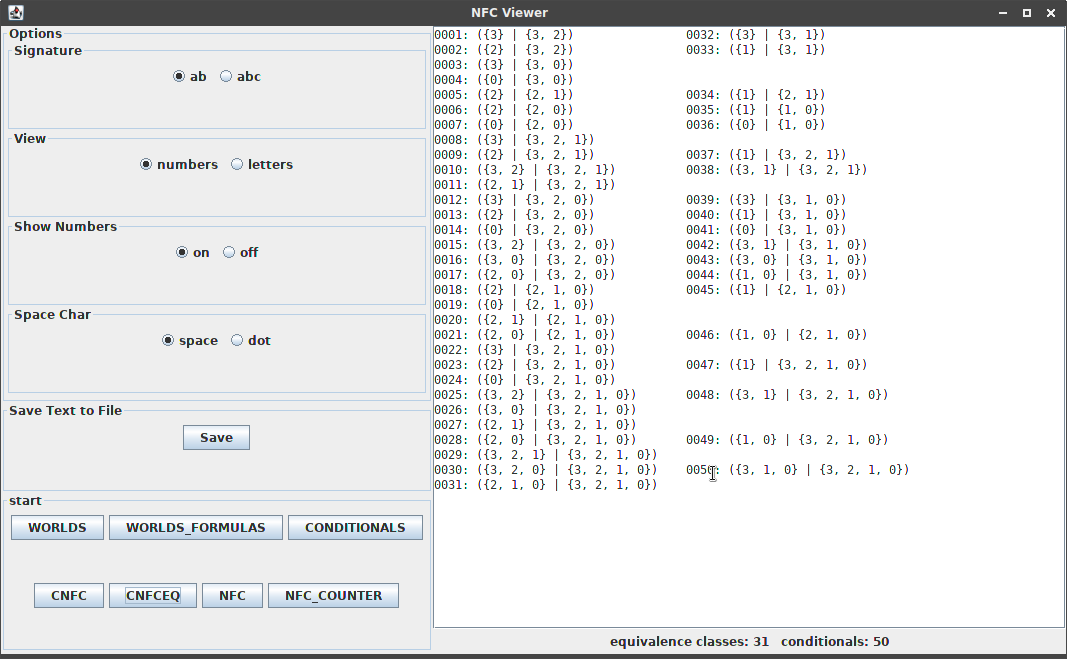
\includegraphics[width=0.8\linewidth]{bilder/nfc-viewer.png}

\caption{Screenshot NFC Viewer mit Ansicht analog zu Tabelle 1 aus \cite{beierle19}}
\label{nfc-viewer}
\end{figure}
Dieses Programm und die dahinterliegende Logik wird in diesem Abschnitt in den folgenden teilen vorgestellt. Das Programm an sich ist nach dem Model View Controller Schema aufgebaut. Die Betrachtung fokussiert sich dabei auf das fachliche Modell dahinter und da, wo es sich anbietet auf die Bedienung und Präsentation dessen auf der Grafischen Oberfläche. Die Logik der Gui und des Controllers werde nicht beschrieben, da sie für das fachliche Thema uninteressant sind. \\
Der Grundsätzliche Aufbau der Gui besteht aus zwei Teilen. Links befinden sich im Oberen Bereich die Optionenauswahl, darunter unter Start befinden sich die Buttons mit den möglichen Aktionen. Auf der rechten Seite Befindet sich ein Textfenster, was das Ergebnis der gewählten Optionen und Aktion zeigt sowie darunter einer kurzen Beschreibung des Inhalts des Textfelds.

\subsection{Mögliche Welten}

Erstellung, Comparable, Auflistung für AB und Nennung ABC?. Äquivalenzklassen und Berechnung der Äquivalenzklassen.

auch was zu eqivalenz, damit auch worldsDifference und WorldsPair.
 Auch zu compare und comparable (hier zum ersten mal)
\subsection{Die Klasse WConditional}
\begin{figure}[h]
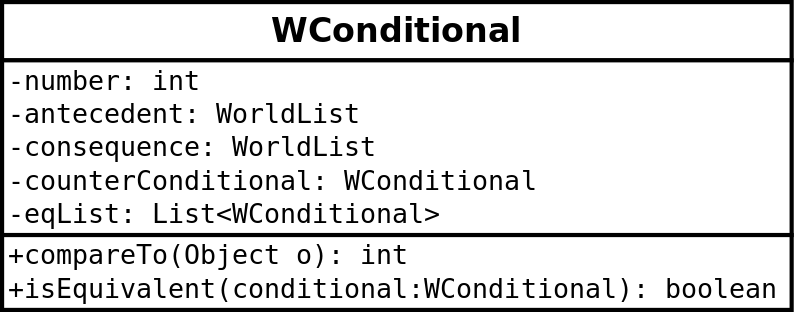
\includegraphics[width=0.45\linewidth]{bilder/wconditional.png}
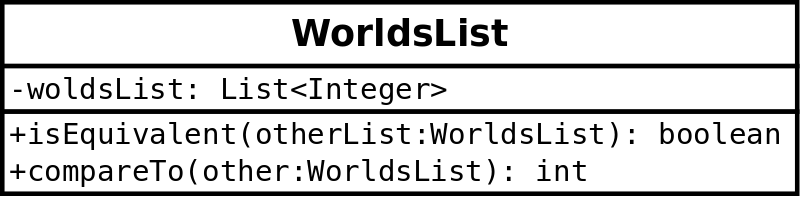
\includegraphics[width=0.45\linewidth]{bilder/worldslist.png}

\caption{WConditional}
\label{wconditional}
\end{figure}

Die Klasse WConditional bildet die Basis für dasGgenerieren der Konditionale aus einer vorgegebenen Signatur. Der Fokus der Klasse liegt dabei auf der Generierung, Ordnung und Betrachtung der Äquivalenz der Konditionale. Ein vereinfachtes Diagramm der Klasse ist in \autoref{wconditional} zu sehen. Attribute der Klasse sind Nummer, CounterConditional und die Liste von äquivalenten Konditionalen. \\
todo: methoden. compareTo(implements comparable!) und isEquivalent() \\
Antecedent und Consequence sind als Objekt der Klasse WorldsList implementiert. Diese Klasse ist gleich daneben in \autoref{wconditional} abgebildet. Sie ist im Prinzip eine Liste mit Nummern der enthaltenen möglichen Welten, erweitert um je einer Methode zum Test von Äquivalenz und zur Sortierung.

\subsection{NFC}
Hier wieder die Ordnung angeben. Wie funktioniert eigentlich die Sortierung nach den verschiedenen möglichkeiten der Sortierung? Kommt das auch nicht durcheinander?
\subsection{cNFC und Äquivalenzklassen}

\section{Konditionale mit Aussagenlogik}
\subsection{Die Klasse PConditional}
Klassendiagramm wär nice.
\subsection{Implemetierung der Aussagenlogik}
Angelehnt an InfOCF \\
Klassen: \\
AbstractFormula\\
->abstract evaluate (always overridden)\\
->concrete equals (never overridden)\\
Atom\\
Negation\\
Conjunction\\
Disjunction\\
\subsection{Übersetzung der Konditionale}
Simple Übersetzung der WorldsList in Disjunctions. Performance Vergleich mit kurzen Übersetzungen als Begründung warum die nicht verwendet werden.
\subsection{Wissensbasen}
Beschreibung der Klasse KnowledgeBase. Klassendiagramm. Für eine entscheiden? Werden überhaupt noch mehrere verwendet?
\section{Beschreibung des Programms Knowledge Base Creator}
\subsection{Aufbau}
Hier ein schönes Übersichtsdiagramm. Hier auch was zum Threading.
\subsection{Implementierung von GenKB}
Erstmal Simple Creator. Funktioniert Parallel? Das wär gut, auch zum gegenüberstellen.
\subsection{Weitere Klassen}
PairBuffer. Pair an sich. Writer. Parallel Writer?
\subsection{Beschreibung der Grafischen Oberfläche}


\section{Generierung der Wissensbasen}
\subsection{Vorüberlegungen}
Wissensbasen sollten in Normalform vorliegen. Siehe dazu auch \cite{beierle17b}. Soll das hier rein oder mit in Grundlagen??
\subsection{Implementierung des Algorithmus}
\subsection{Generierung der Wissensbasen}
\subsection{Darstellung des Ergebnisses}
\section{Bewertung der Ergebnisse}

\newpage
\bibliographystyle{alpha}
\bibliography{lit} 
\end{document}